\subsection*{SIERD + вакцинация}
\addcontentsline{toc}{subsection}{SIERD + вакцинация}

\textbf{Задание:}\\
Реализовать модель распространения заболевания с добавлением новых состояний: носитель заболевания, умершие и вакцинированные.\\

\textbf{Решение:}\\
Данная модель реализуется похожую логику на ту которая была в модели SIR, поэтому в данном разделе будут рассмотренны только модификации.\\

В качестве новых параметров добавились вероятность вакцинации, вероятность выжить и время, которое должно пройти с момента вакцинации, чтобы вакцина успела подействовать.\\

Диаграмма состояний в таком случае будет изменена и примет следующий вид.  (Рисунок \ref{fig:sierd1})
\begin{figure}[h]
	\centering 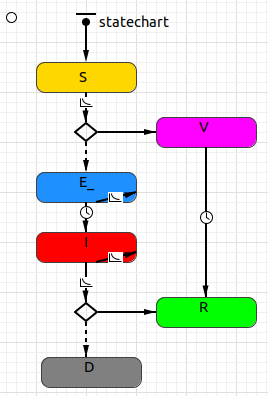
\includegraphics[scale=0.5]{sierd1}
	\caption{Диаграмма состояний}
	\label{fig:sierd1}
\end{figure}

Теперь из состояния когда человек полностью здоров можно перейти в состояние, когда человек вакцинирован или является носителем. Данный переход происходит с вероятностью, для которой был введён отдельный параметр. Если агент вакцинировался, то он сразу же попадает в состояние -- выздоровевший.\\

Если же человек стал носителем, то дальше через некоторое время он заболевает, и в процессе пока он является носителем он также может заражать других здоровых людей. Далее из состояние больного агент может перейти в состояние умершего или выздоровевшего с заданной вероятность. Для этого был введён специальный параметр, который рассмотрен чуть выше.\\

В результате работы данной модели был получен график, который похож, на тот, что мы рассматривали на системной динамике. (Рисунок \ref{fig:sierd2})
\begin{figure}[h]
	\centering 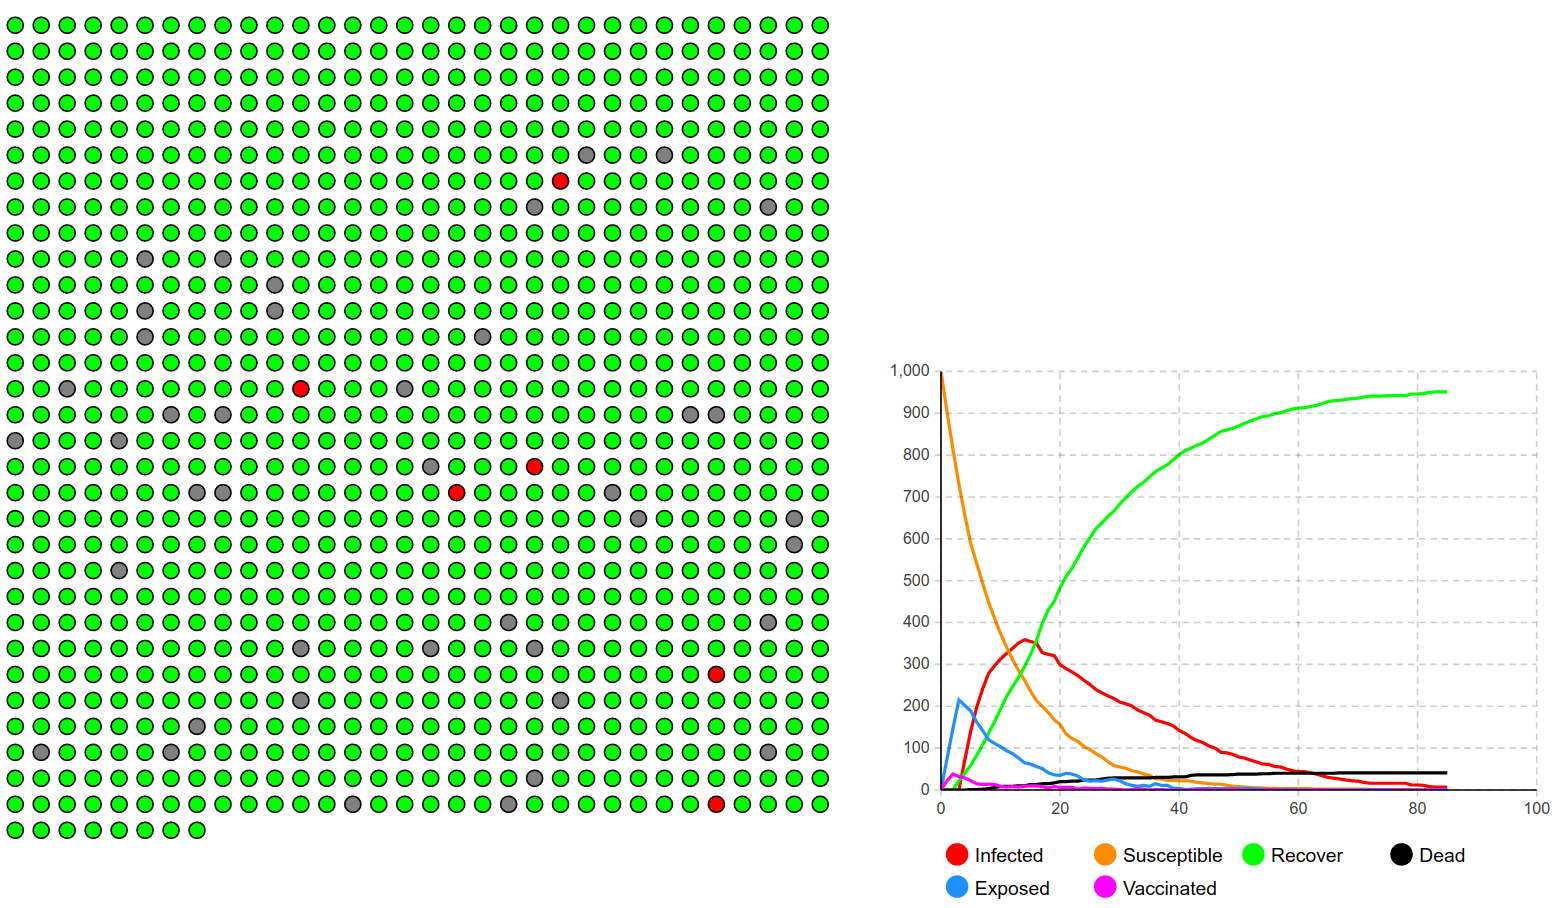
\includegraphics[scale=0.3]{sierd2}
	\caption{Результат модели SIERD}
	\label{fig:sierd2}
\end{figure}

Таким образом, посредством агентного моделирования была построена модель распространения заболевания с учётом вакцинации.